\chapter{Produktfunktionen}

\textbf{Produktfunktionen}
\section{/LF10/ Hardware und Sensorik}
Geschäftsprozess:	Verarbeitung der Sensordaten
Akteur:			CarPC
Beschreibung:	Aufbau von Sensoren zur Erfassung von Fahrdaten und Ansteuerung von Schnittstellen zum Motormanagement in einem einfach zu installierenden CarPC.

\textbf{•/LF11/ CarPC}
\nextline
Es soll ein Single Board Computer (SBC) verwendet werden, welcher alle verwendeten Sensoren unterstützt. Die Montage darf den Fahrer nicht behindern. Idealerweise ist der CarPC mobil auszuführen, damit er in mehreren Fahrzeugen verwendet werden kann. Die Stromversorgung muss über das 12V Bordnetz eines Kfz möglich sein, bei Fixeinbau muss diese mit der Zündung gekoppelt werden.

\textbf{•/LF12/Anbindung der ODB Schnittstelle an den CarPC}
\nextline
Der CarPC soll Motordaten aus der standardisierten Diagnoseschnittstelle des Fahrzeugen auslesen können. Diese Motordaten umfassen beispielsweise die Drehzahl des Motors, die Fahrgeschwindigkeit und wenn möglich auch den eingelegten Gang.

\textbf{•LF13 Messung der Fahrzeugbeschleunigung in Fahrzeuglängst- und -querachse}
\nextline
Die Beschleunigung in Fahrzeuglängs- (Beschleunigung und Bremsen) sowie die Fahrzeugquerachse (Kurvenbeschleunigung) sollen in die Verbrauchsinformation und Fahrgastbequemlichkeit einfließen.

\newpage
\textbf{•/LF14/ Messung der Fahrzeugneigung in 3 Raumachsen}
\nextline
Die Drehung des Fahrzeug in alle Raumachsen wird mit dem Gyroskop gemessen. Die Bewegung um die Raumachsen heißen bei einem Kfz Kippen, Rollen und Gieren. Diese Informationen werden in weiterer Folge vor allem für die Erkennung eines Hangs eingesetzt, aber auch für die Fahrgastbequemlichkeit.

\textbf{•/LF15/ Messen der geographischen Fahrzeugposition}
\nextline
Ein GPS Sensor muss am CarPC angeschlossen sein um den Standort des Fahrzeugs ermitteln zu können und um die Verbrauchs- und Neigungswerte kartieren zu können.

\textbf{•/LF 16/ Messung des Fahrgastraumklimas}
\nextline
Ein Temperatursensor und mögliche weitere Sensoren werden im CarPC integriert um die Fahrgastbequemlichkeit besser beurteilen zu können.

\textbf{•/LF17/ Multifahrzeug-Management}
\nextline
Der Benutzer soll die Möglichkeit haben, ein Fahrzeugprofil auszuwählen (in Verbindung mit der Android-App). Damit soll eine mehrfache Verwendung des CarPCs (so eine mobile Lösung implementiert wurde) in verschiedenen Fahrzeugen gewährleistet werden.
\newpage

\section{/LF20/ Datenmanagement und Datenanalyse}
\textbf{Geschäftsprozess:}	Verarbeitung der Sensor Daten
\newline
\textbf{Akteur:}		CarPC, standardisierte informationsschnittstelle
\newline
\textbf{Beschreibung:} Aufbereitung und effiziente Speicherung von Daten verschiedener Fahrzeugsensoren und Implementierung von Schnittstellen für weitere Applikationen. 

\textbf{•/LF21/ Sammlung und Speicherung aller Sensordaten und Ablegen in einer strukturierten Form}
\nextline
Die Sensordaten müssen gesammelt und so gespeichert werden, dass sie strukturiert und zur Weiterverarbeitung vorbereitet sind.

\textbf{•/LF22/ Interpretation der Rohdaten in Messgrößen mit gängigen Einheiten}
\nextline
Alle Rohdaten müssen in einen normierten Wert in einer sinnvollen Einheit umgewandelt werden. Dabei ist besonders zu beachten, ob und wie die Positionierung der Sensoren im Fahrzeug auf die Messwerte einen Einfluss hat.

\textbf{•/LF23/ Filterung von offensichtlichen Messfehlern}
\nextline
Bei dieser Funktion ist vor allem die Auswahl was als Messfehler gewertet wird entscheidend. Denn es sollen zwar Messfehler gefunden und entfernt werden, allerdings sollen auch die Maxima der wirklichen Fahrt nicht fälschlicher Weise gefiltert werden. Daher hängt diese Filterung auch sehr nahe mit der Interpretation der Rohdaten zusammen.

\textbf{•/LF24/ Zusammenfassung von Messgrößen}
\nextline
Zur einfacheren Weiterverarbeitung sollen Messwerte (wo sinnvoll) schon vom CarPC sinnvoll vorverarbeitet und zusammengefasst werden.

\textbf{•/LF25/ Implementierung einer Schnittstelle zur Kommunikation mit der Android App}
\nextline
Die auf dem CarPC gesammelten Daten müssen sich einfach von der Android-App (siehe LF30/40/50) abrufen lassen. Dafür muss eine Schnittstelle entwickelt werden, die energieeffiezient arbeitet, aber auch schnell genug ist, Momentanwerte zeitgerecht zu übertragen.
\newpage

\section{/LF30/ Schaltvorgangsvorschlag}
Geschäftsprozess:	Algorithmus zur Berechnung des Kraftstoff sparenden Schaltvorgangs, Algorithmus zur Berechnung des leistungsstärksten Schaltvorgangs
Akteur:			App, standardisierte Informationsschnittstelle
Beschreibung:	Auswertung von Fahrdaten in einer Android App, um dem Fahrer visuell und akustisch einen Vorschlag für einen effizienten Schaltzeitpunkt zu geben. 

\textbf{•/LF31/ umweltschonenden Schaltvorschlag ermitteln}
\nextline
Der Schaltvorschlag soll so berechnet werden, dass eine Befolgung sich möglichst positiv auf den Kraftstoffverbrauch auswirkt und dadurch Kosten gespart und die Umweltbelastung gesenkt werden.

\textbf{•/LF32/ Schaltvorschlag für maximales Drehmoment ermitteln}
\nextline
Der Schaltvorschlag soll so berechnet werden das laut der Leistungskurve ein hohes Drehmoment gewährleistet bleibt. 

\textbf{•/LF33/ Einbindung der Fahrzeugneigung in die Ermittlung Schaltvorschläge }
\nextline
Es wird mittels des Gyroskops festgestellt ob sich das Fahrzeug auf einer Steigung oder auf einem Gefälle befindet, auf Basis dieser Information wird dann entschieden ob der Schaltvorgang vorgeschlagen werden soll, um einen Nutzer nicht mitten auf einem Gefälle bei der Benutzung der Motorbremswirkung zu behindern. 

\textbf{•/LF34/ Audiovisuelle Schaltaufforderungen}
\nextline
Der Fahrer soll über einen Schaltvorschlag visuell und/oder auditiv, möglichst ablenkungsfrei, informiert werden. Dies könnte einerseits mit einer Sprachausgabe und andererseits mit einem Schaltlicht und einer simplen Anzeige realisiert werden. Der Benutzer soll dies auch teilweise konfigurieren können (z.B: Ton ausschalten)

Hier sind die Icons die angezeigt werden um den Fahrer audiovisuell zu benachrichtigen.                                                                    Er sollte auch die Möglichkeit haben die Buttons anzuklicken um den Ton auszuschalten. 

\newpage
\section{/LF40/ Verbrauchsanalyse}
Geschäftsprozess:	Analyse des Kraftstoffverbrauchs
Akteur:			App, standardisierte Informationsschnittstelle, Datenbank
Beschreibung:	Auswertung und visuelle Aufbereitung von Fahrdaten in einer Android App, um Tipps und Feedback zu einer kraftstoffsparenden Fahrweise zu geben.

\textbf{•/LF41/ Fahrmodus: Anzeige des Momentanverbrauchs und Durchschnittsverbrauchs der Strecke}
\nextline
Die Anzeige muss großflächig und gut ablesbar sein, siedarf  keine Ablenkung beim Lenker des KFZ hervorrufen. 
Große Zahlen

\textbf{•/LF42/ Fahrmodus: Audiovisuelle Tipps zur verbrauchsbezogenen Veränderung des Fahrverhaltens}
\nextline
Visuell mittels Veränderung der visuellen Gestaltung der App, auditiv mit in der App einzigartigem Warnsignal.

\textbf{•/LF43/ Analysemodus: Anzeige des Verbrauchsverlaufs über die Zeit/Fahrstrecke linear und Fahrstrecke geographisch}
\nextline
Es soll eine Analysemöglichkeit in der App eingebaut werden, welche dafür verwendet werden kann um eine Fahrt bezüglich Verbrauch, Geschwindigkeit und anderen Werten Revue passieren zu lassen. Zusätzlich sollen Informationen welche besonders herausstechen in einem Diagramm und auf einer Karte der Route besonders hervorgehoben werden. Um die Menge der Analysedaten zu reduzieren, sollen ältere Streckeninformationen nur mehr aggregiert zur Verfügung stehen (d.h. die „Auflösung“ der Information nimmt mit zunehmenden Alter der Daten ab). Möchte der Benutzer Daten zu bestimmten Strecken erhalten, so soll eine Exportmöglichkeit geboten werden.

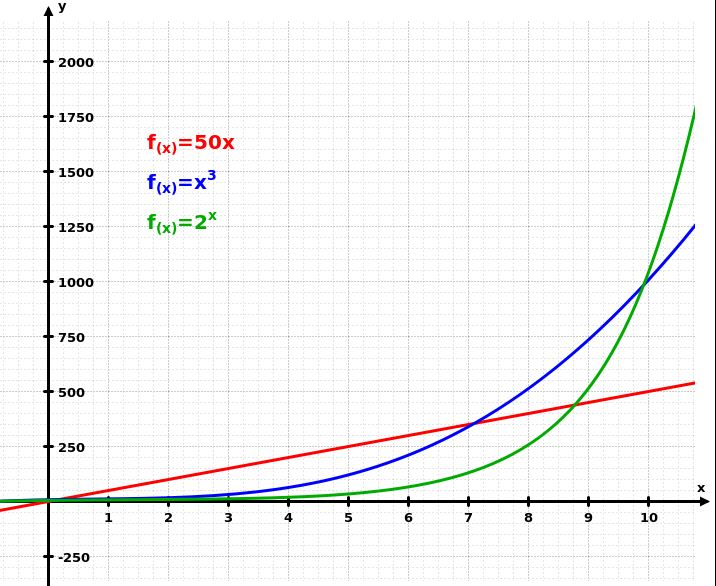
\includegraphics{images/LF43_Diagramm.jpg}

Hier Wird der Verbrauchsverlauf dargestellt auf der x Achse wird die Zeit eingetragen und auf der y Achse der CO2 Ausstoß

\textbf{•/LF44/ Analysemodus: Vergleichsmöglichkeit des Verbrauchsverlaufs über mehrere Strecken}
\nextline
Es gilt zu evaluieren ob diese Vergleichsmöglichkeit nur in der App implementiert werden soll, oder ob diese auch in einer Desktop Version entwickelt werden sollte.

\textbf{•/LF45/ Analysemodus: Upload eines kommentierten Verbrauchsverlaufs auf SocialMedia-Plattformen }

\newpage

\section{/LF50/ Fahrkomfortanalyse}
Geschäftsprozess:	Analyse verschiedener Fahrdaten in Bezug auf die Fahrgastbequemlichkeit.
Akteur:			App und standardisierte Informationsschnittstell
Beschreibung:	

Auswertung und visuelle Aufbereitung von Fahrdaten in einer Android App, um Tipps und Feedback über den Fahrkomfort seines Fahrverhaltens zu geben.

\textbf{•/LF51/ Fahrmodus: Visualisierung der momentanen Beschleunigungskräfte}
\nextline
Es soll eine Anzeige der momentanen Beschleunigungskräfte mittels einer intuitiv ablesbaren Visualisierung angezeigt werden (beispielsweise kammscher Kreis)
\nextline
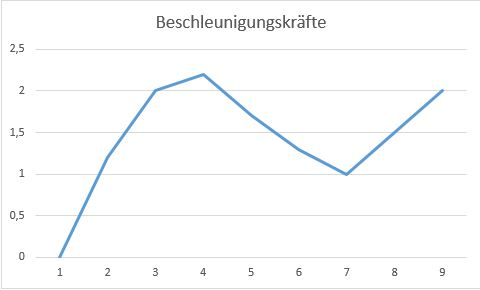
\includegraphics{images/LF51_Beschleunigung.jpg}
\nextline
Die Grafik für die Anzeige der Beschleunigungskräfte würde ungefähr so aussehen

\textbf{•/LF52/ Fahrmodus: Audiovisuelle Tipps zur Veränderung des Fahrverhaltens im Bezug auf die Fahrgastbequemlichkeit.}
\nextline
Dem Fahrer sollen Tipps zur Erhöhung des Fahrgastkomforts gegeben werden können. Mögliche Umsetzungen: Hinweis auf zu hohe Querbeschleunigungen, Geschwindigkeitsvorschläge aufgrund des zu erwartenden Straßenverlaufs, Umwelteinflüsse im Fahrgastraum.
Hier sind die Icons die angezeigt werden um den Fahrer audiovisuell zu benachrichtigen.                                                                    Er sollte auch die Möglichkeit haben die Buttons anzuklicken um den Ton auszuschalten. 
\nextline
\textbf{•/LF53/ Analysemodus: Anzeigen der Beschleunigungen einer Fahrt }
\nextline
Analog zu LF43 sollen die Beschleunigungsdaten einer Fahrt linear und ortsbezogen in verschiedenen Visualisierungen analysiert werden können.
\nextline
 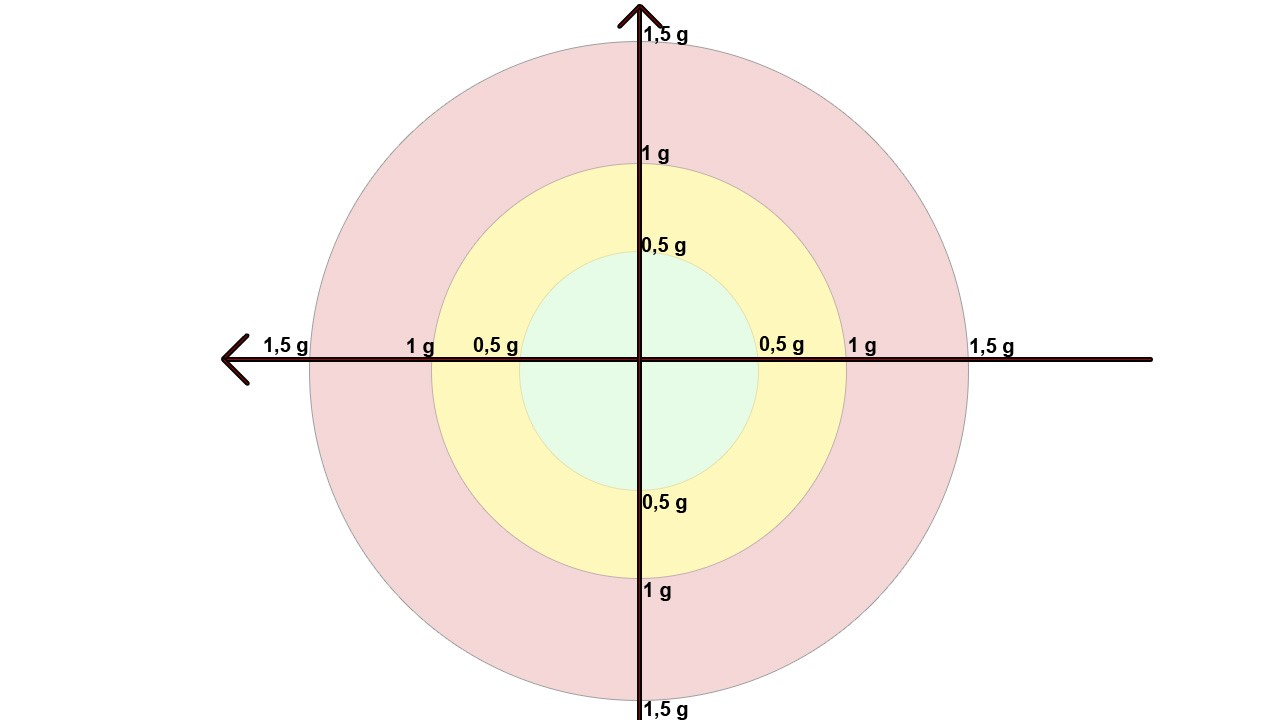
\includegraphics[scale=0.3]{images/LF53_Kalm.jpg}
 \nextline
Hier wird das mittels eines Kammschen Kreis verwirklicht, welcher mit mehreren Punkten gefüllt wird wodurch sich eine Fläche bildet, die Kreise sind die Grenzen der Beschleunigungskräfte

\textbf{•/LF54/ Analysemodus: Vergleichsmöglichkeit mit früheren Fahrten}
\nextline
Es soll hierfür die Möglichkeit geben, Diagramme zu überlagern, sowie Karten-Overlays zu überlagern 
\nextline
 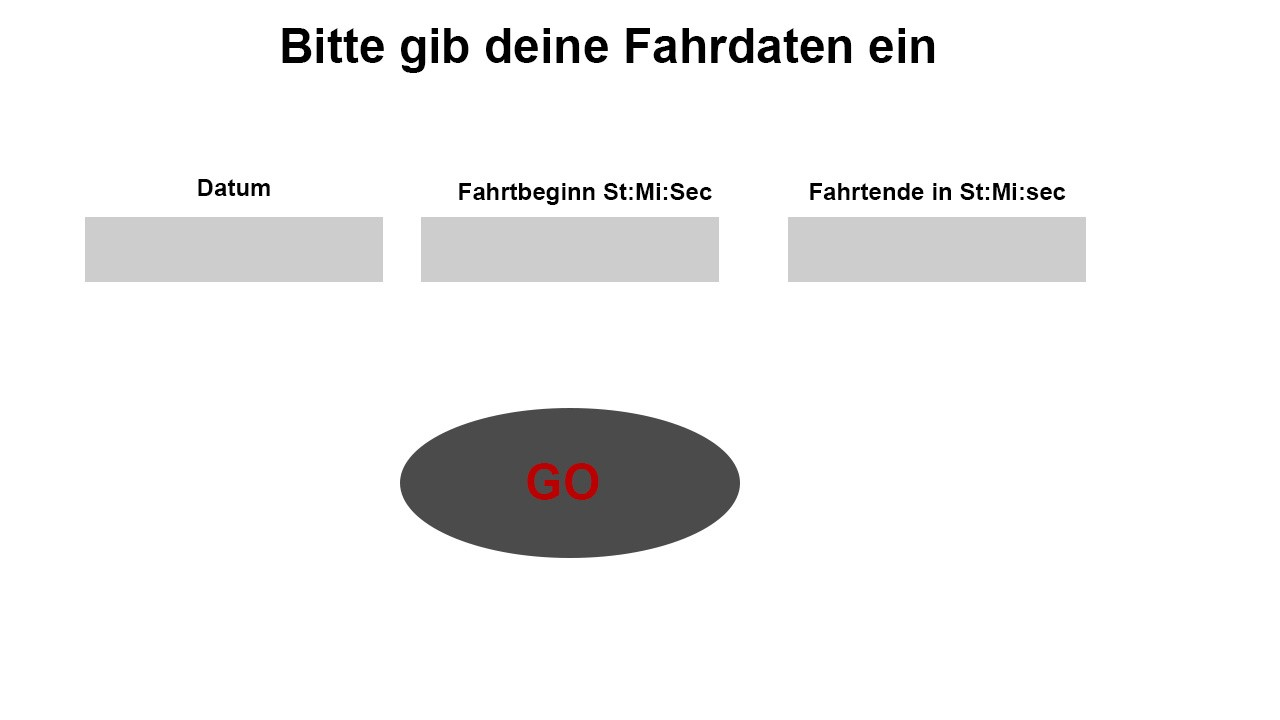
\includegraphics[scale=0.3]{images/LF54_Fahrdaten.jpg}
 \nextline
Mittels einer Eingabe einer Bestimmten Fahr können Grafiken gespeichert und später gegenüber gestellt werden. 

\newpage

\section{/LF90/ Android App}
Geschäftsprozess:	Benutzerfreundlichkeit der App, Rechtliche Absicherung
Akteur:			App, standardisierte Informationsschnittstelle
Beschreibung:	Aufbereitung und effiziente Speicherung von Daten verschiedener Fahrzeugsensoren und Implementierung von Schnittstellen für weitere Applikationen. 
Die App würde ungefähr so ausschauen, dass der Benutzer vor sich etwas größere Knöpfe hat,                                        
womit er von einer Funktion zu der anderen springen kann.

\textbf{•/LF91/ Warnmeldung bei Appstart}
\nextline
Es muss eine Warnmeldung beim Start der App eingeblendet werden um dem Nutzer darüber in Kenntnis zu setzen, dass die Straßenverkehrsordnung in jedem Fall zu beachten ist und die Beschilderung auf der Straße immer beachtet werden muss (siehe andere Navigationsgeräte).

Beim Starten der App sollte der Fahrer darauf aufmerksam gemacht werden, dass die App ihn nicht zum schnell Fahren anstiftet soll dafür wird ein Text eingeblendet
\emph{„Die Macher und Entwickler dieser App haften für nichts, wird bitten sie die Straßenverkehrsordnungen zu befolgen, um alle andere Fahrer nicht zu gefährden „}

\textbf{•/LF92/ Streckenverwaltung implementieren}
\nextline
Zu Beginn der Benutzung der App soll der Nutzer entscheiden können ob er eine neue Strecke mit dieser Fahrt beginnen will, oder ob er seine letzte Fahrt an diesem Ort weiterführen möchte.

\textbf{•/LF93/ Konfigurieren von Fahrzeugparametern}
\nextline
Der User soll für die Funktion der App notwendige Konfigurationsdaten hinterlegen können. Dazu werden vermutlich auch einige Fahrzeugparameter gehören, sofern diese nicht automatisch aus dem Fahrzeugmanagement gelesen werden können. Diese Daten sollen in einem Profil abgelegt werden können..

Könnte ungefähr wie be den Fahrdaten aussehen 

\textbf{•/LF94/ Multifahrzeug-Management}
\nextline
Der Benutzer soll die Möglichkeit haben, ein Fahrzeugprofil auszuwählen. Damit soll eine mehrfache Verwendung der App in verschiedenen Fahrzeugen gewährleistet werden.

\textbf{• /LF99/ Integration von OpenStreetMaps um vorrausschauend Tipps für das Fahverhalten geben zu können}
\nextline
Es gilt zu evaluieren ob eine Einbindung von Kartendaten möglich wäre um beispielsweise Steigungen vorherzusagen, um vor einer Steigung auf einen niedrigeren Gang zu wechseln, damit der Motor nicht mit geringer Leistung und hohem Gang den Berg befahren muss, sondern die Fahrzeugkomponenten geschont werden indem vorher zurück geschalten wird. Besonders praktisch wären diese Daten z.B. besonders bei engen Kurven um einen empfohlenen Gang/Geschwindigkeit für eine Kurve vorzuschlagen.
